\documentclass[10pt, a5paper]{article}
\usepackage{pdfpages}
\usepackage{parallel}
\usepackage[T2A]{fontenc}
\usepackage{ucs}
\usepackage[utf8x]{inputenc}
\usepackage[polish,english,russian]{babel}
\usepackage{hyperref}
\usepackage{rotating}
\usepackage[inner=2cm,top=1.8cm,outer=2cm,bottom=2.3cm,nohead]{geometry}
\usepackage{listings}
\usepackage{graphicx}
\usepackage{wrapfig}
\usepackage{longtable}
\usepackage{indentfirst}
\usepackage{array}
\newcolumntype{P}[1]{>{\raggedright\arraybackslash}p{#1}}
\frenchspacing
\usepackage{fixltx2e} %text sub- and superscripts
\usepackage{icomma} % коскі ў матэматычным рэжыме
\PreloadUnicodePage{4}

\newcommand{\longpage}{\enlargethispage{\baselineskip}}
\newcommand{\shortpage}{\enlargethispage{-\baselineskip}}

\def\switchlang#1{\expandafter\csname switchlang#1\endcsname}
\def\switchlangbe{
\let\saverefname=\refname%
\def\refname{Літаратура}%
\def\figurename{Іл.}%
}
\def\switchlangen{
\let\saverefname=\refname%
\def\refname{References}%
\def\figurename{Fig.}%
}
\def\switchlangru{
\let\saverefname=\refname%
\let\savefigurename=\figurename%
\def\refname{Литература}%
\def\figurename{Рис.}%
}

\hyphenation{admi-ni-stra-tive}
\hyphenation{ex-pe-ri-ence}
\hyphenation{fle-xi-bi-li-ty}
\hyphenation{Py-thon}
\hyphenation{ma-the-ma-ti-cal}
\hyphenation{re-ported}
\hyphenation{imp-le-menta-tions}
\hyphenation{pro-vides}
\hyphenation{en-gi-neering}
\hyphenation{com-pa-ti-bi-li-ty}
\hyphenation{im-pos-sible}
\hyphenation{desk-top}
\hyphenation{elec-tro-nic}
\hyphenation{com-pa-ny}
\hyphenation{de-ve-lop-ment}
\hyphenation{de-ve-loping}
\hyphenation{de-ve-lop}
\hyphenation{da-ta-ba-se}
\hyphenation{plat-forms}
\hyphenation{or-ga-ni-za-tion}
\hyphenation{pro-gramming}
\hyphenation{in-stru-ments}
\hyphenation{Li-nux}
\hyphenation{sour-ce}
\hyphenation{en-vi-ron-ment}
\hyphenation{Te-le-pathy}
\hyphenation{Li-nux-ov-ka}
\hyphenation{Open-BSD}
\hyphenation{Free-BSD}
\hyphenation{men-ti-on-ed}
\hyphenation{app-li-ca-tion}

\def\progref!#1!{\texttt{#1}}
\renewcommand{\arraystretch}{2} %Іначай формулы ў матрыцы зліпаюцца з лініямі
\usepackage{array}

\def\interview #1 (#2), #3, #4, #5\par{

\section[#1, #3, #4]{#1 -- #3, #4}
\def\qname{LVEE}
\def\aname{#1}
\def\q ##1\par{{\noindent \bf \qname: ##1 }\par}
\def\a{{\noindent \bf \aname: } \def\qname{L}\def\aname{#2}}
}

\def\interview* #1 (#2), #3, #4, #5\par{

\section*{#1\\{\small\rm #3, #4. #5}}

\def\qname{LVEE}
\def\aname{#1}
\def\q ##1\par{{\noindent \bf \qname: ##1 }\par}
\def\a{{\noindent \bf \aname: } \def\qname{L}\def\aname{#2}}
}

\switchlang{ru}
\begin{document}
\title{Безопасноcть в браузерах: Альтернативы SSL\footnote{\url{alexei.khlebnikov@gmail.com}, \url{http://lvee.org/ru/abstracts/249}}}
\author{Алексей Хлебников, Oslo, Norway}
\maketitle
\begin{abstract}
Browser makers spend a lot of effort for making SSL right and make PKI
harder then ever, but pay too little attention to alternative methods
of estimating the web site security. In this talk I will tell about
such alternative methods and a little bit about using risk management
for security level estimation.
\end{abstract}
\subsection*{Ожидания и реальность}

На первых этапах внедрения SSL в Web, на SSL возлагались большие
надежды. Предполагалось, что будет примерно так:

\begin{center}

\begin{figure}[h!]
  \centering
  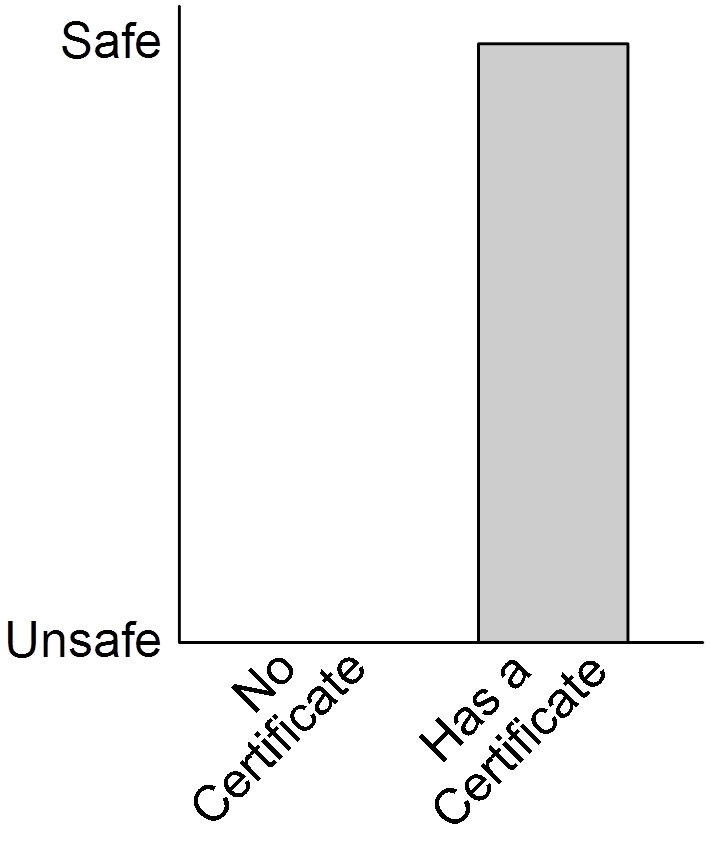
\includegraphics[width=4cm]{Hlebnikov1.png}
  \caption{SSL-безопасность в Web: что предполагалось}
  \label{Hlebnikov1}
\end{figure}

\end{center}

Однако, реальность оказалась сложнее. Например, пользоваться SSL стали
и компьютерные преступники.

Cкриншот с форума, где DDOS-еры предлагают свои услуги: 

\begin{center}

\begin{figure}[!h]
  \centering
  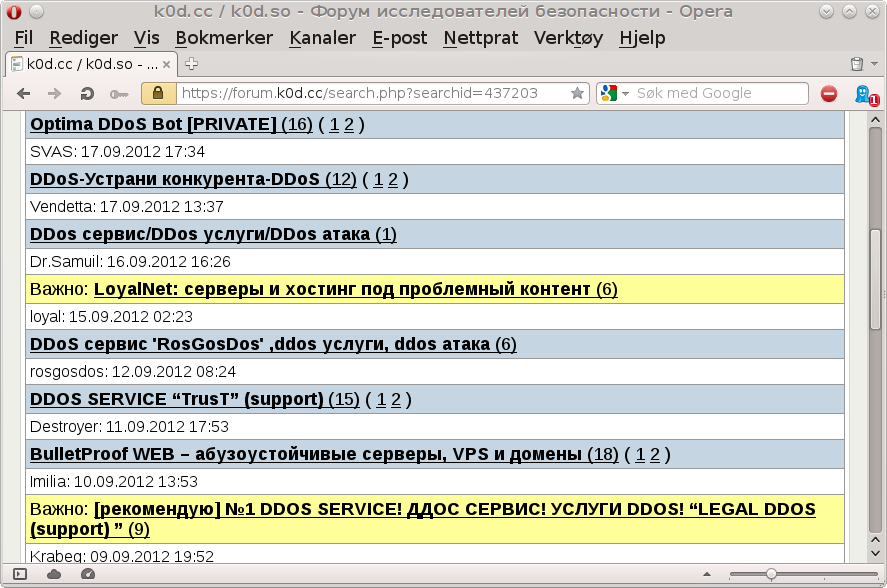
\includegraphics[width=10cm]{Hlebnikov2.png}
 \caption{Форум киберпреступников, на котором предлагаются услуги DDOS. SSL-сертификат успешно прошёл проверку}

  \label{Hlebnikov2}
\end{figure}

\end{center}

Как видно, SSL-сертификат успешно проверен, замочек показан.
Пользователь может быть уверен, с сайтом <<всё в порядке>>.

%А вот скриншот с сайта visa.com:

\begin{center}
\begin{figure}[!h]
  \centering
  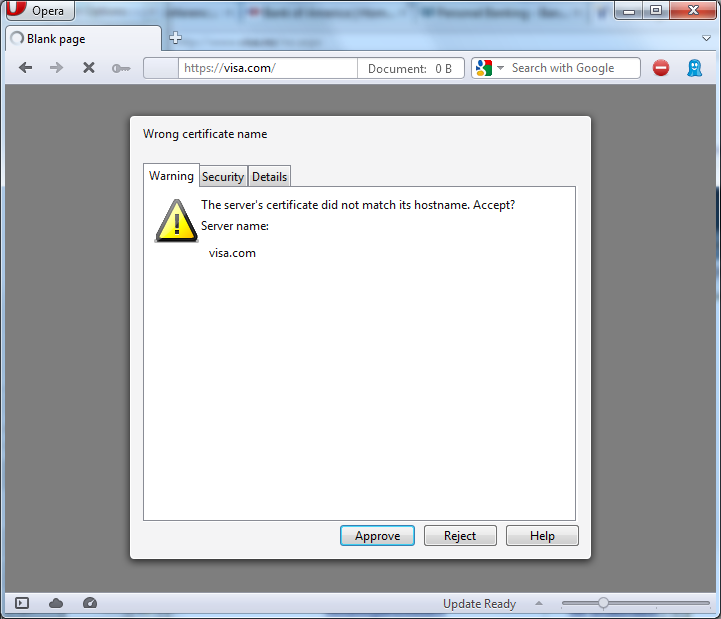
\includegraphics[width=10cm]{Hlebnikov3.png}
  \caption{Сайт платёжной системы Visa. SSL-сертификат не прошёл проверку}
  \label{Hlebnikov3}
\end{figure}
\end{center}

Видим, что сертификат браузеру определённо не нравится ~\ref{Hlebnikov3}. Внимательный
читатель наверное уже догадался, что сертификат выписан на имя
<<www.visa.com>>, а введённый адрес ~--- просто <<visa.com>>, без префикса
<<www>>. Но обычный пользователь вряд ли это поймёт, а вполне может
подумать, что его атакуют.

Совсем плохо приходится некоммерческим CA. Их сертификаты будут
признаны недействительными без ручной установки в браузер, а значит
у большинства пользователей. Браузер отвергает даже сам сайт такого
CA ~\ref{Hlebnikov4}:

\begin{center}
\begin{figure}[h!]
  \centering
  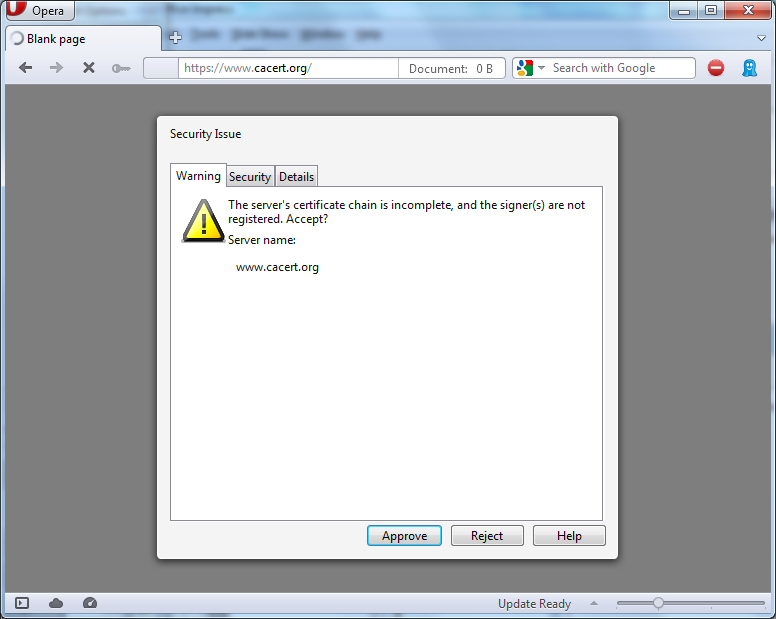
\includegraphics[width=10cm]{Hlebnikov4.png}
  \caption{Сайт некоммерчесского CA. SSL-сертификат не прошёл проверку}
  \label{Hlebnikov4}
\end{figure}
\end{center}
Заметим, что браузеры совсем не выдают таких предупреждений для
сайтов, которые предоставляются не по HTTPS, а по HTTP, то есть
вообще без сертификата. Таким образом, упрощённая модель
SSL-безопасности в Web выглядит скорее ~\ref{Hlebnikov5}, что не очень логично, так как <<плохой>> сертификат всё-таки лучше его
отсутствия.

\begin{center}
\begin{figure}[h!]
  \centering
  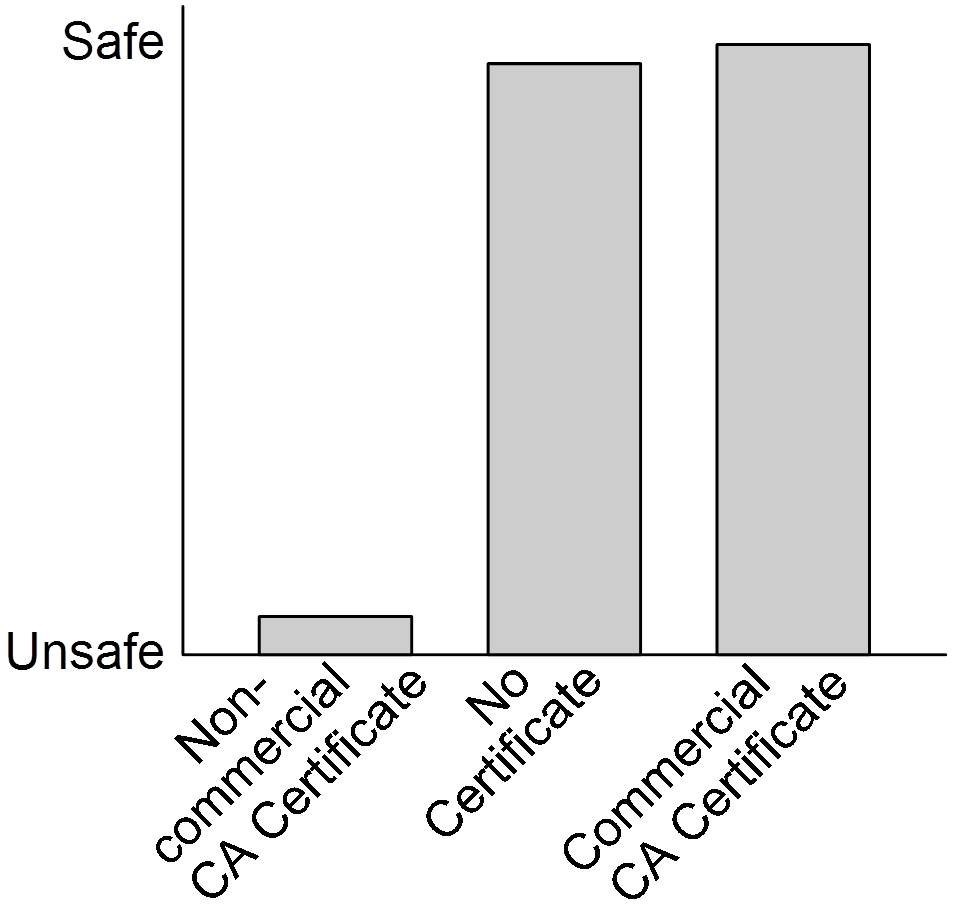
\includegraphics[width=6cm]{Hlebnikov5.png}
  \caption{SSL-безопасность в Web: что получилось}
  \label{Hlebnikov5}
\end{figure}
\end{center}

Логичнее было бы ~\ref{Hlebnikov6}.
\begin{center}
\begin{figure}[h!]
  \centering
  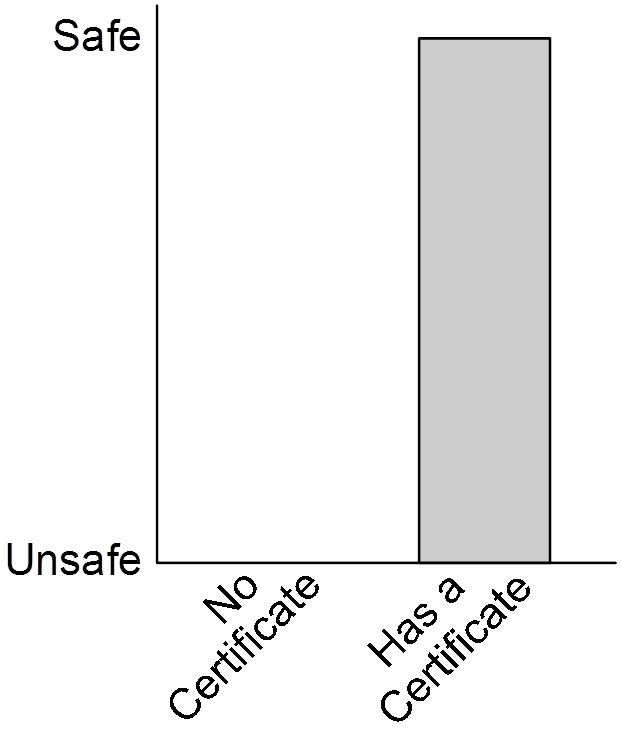
\includegraphics[width=6cm]{Hlebnikov6.png}
  \caption{SSL-безопасность в Web: что было бы логичнее}
  \label{Hlebnikov6}
\end{figure}
\end{center}
\subsection*{Взломы SSL}

На этом проблемы SSL не заканчиваются. За прошедшие годы случались
инциденты и взломы CA-инфраструктуры. Вот их неполный список:

\begin{itemize}
  \item 2001 ~--- Атакующий прикинулся сотрудником Microsoft и получил у
  Verisign сертификат для Microsoft.
  \item 2008 ~--- На сервисе live.com зарегистрирован бесплатный e-mail
  sslcertificates@live.com, затем у Thawte получен сертификат для
  login.live.com.
  \item 2008 ~--- Взломы StartCom и Comodo, у Comodo получен сертификат для
  www.mozilla.com.
  \item 2009 ~--- Взлом ipsCA через NULL prefix attack, получен сертификат для
  www.paypal.com.
  \item 2011 ~--- Взломы Comodo, Diginotar и TurkTrust. Получены сертификаты
  для \url{www.google.com}, \url{mail.google.com}, \linebreak \url{addons.mozilla.org},
  \url{login.live.com}, \url{login.yahoo.com}, \linebreak \url{login.skype.com}. Шуточная атака
  <<Honest Achmed>> на Mozilla.
  \item 2014 ~--- Взлом NICCA, получены сертификаты для доменов Google и Yahoo.
  \item 2015 ~--- Взломы CNNIC, WoSign, Let's Encrypt и Symantec. Получены
  сертификаты для доменов Google, GitHub и других.
  \item 2016 ~--- Найдены уязвимости в инфрастркутурах выдачи сертификатов у
  StartCom и Comodo. Были ли эти уязвимости использованы и как ~--- пока
  неизвестно.
\end{itemize}

А также взломы разной степени эффективности самого протокола SSL/TLS:

\begin{itemize}
  \item 2009 ~--- Renegotiation attack, SSL stripping.
  \item 2011 ~--- BEAST, StartTLS injection.
  \item 2012 ~--- CRIME.
  \item 2013 ~--- BREACH, TIME, Lucky13.
  \item 2014 ~--- FREAK, POODLE, Triple Handshake.
  \item 2016 ~--- DROWN.
\end{itemize}

А также не будем забывать о периодически находимых уязвимостях в
реализациях SSL, например Heartbleed в OpenSSL.

\subsection*{Система CA недостаточно надёжна}

До сих пор никто так и смог дать убедительного ответа, почему сайты и
пользователи должны доверять тем самым CA, которых большинство
пользователей в глаза не видело. Ответ <<по умолчанию>> на этот вопрос -
потому что CA берут деньги за выдачу сертификата, и если они вдруг
выдадут неправильный сертификат или будут взломаны ~--- сразу потеряют
доверие, клиентов и разорятся. Мне в этот аргумент почему-то не
очень-то верится. Особенно в свете известных вышеперечисленных
взломов. Кто из CA понёс серьёзное наказание в результате взлома и
прекратил выдачу сертификатов? Почти никто. Только маленький
Diginotar. А взлом Comodo в том же году, наделавший немало шума -
спустили на тормозах. Потому что Comodo ~--- <<too big to fail>>. Работает
дальше и продолжает <<радовать>> нас периодическими уязвимости своей
инфраструктуры выдачи сертификатов. А сколько взломов не стало
достоянием общественности? А ведь CA довольно неохотно раскрывают
факты взломов своей инфраструктуры, и бывали уличены в сокрытии такой
информации.

А можем ли мы быть уверены, что если в офис CA придут
сотрудники местных спецслужб и попросят выдать им сертификат на не
принадлежащий им домен, то СА откажет им? Скорее, мы можем быть
уверены в обратном. А знает ли уважаемый читатель, что в США полицией
и спецслужбами уже несколько лет используются так называемые MITM
boxes? Это устройство, которое в реальном времени осуществляет
MITM-атаку и расшифровывает весь SSL-траффик, проходящий через
устройство. Причём, пользователь, которого прослушивают, не получает
никаких предупреждений от своего браузера, потому что MITM-box на лету
выдаёт <<правильные>> сертификаты для всех серверов, посещаемых
пользователем. Как устройчтво это делает? Очень просто ~--- устройство
обладает intermediate-CA сертификатом, который любезно выдан крупным
американским CA, которому, конечно, доверяют все браузеры.

Большая проблема здесь ~--- то что абсолютно любой CA может выдать
сертификат абсолютно любому сайту. Это ещё хуже, чем единая точка
отказа. Доверие CA-центрам ~--- абсолютно, а они его, прямо скажем,
не заслужили.

А ещё некоторые CA доверяют выдачу своих сертификатов другим фирмам,
эдаким дилерам. Прямо как подключение телефона в салоне связи. А ещё
многие CA вполне официально выдают некоторым крупным бизнес-клиентам
сертификаты, позволяющие выдавать другие сертификаты, то есть частично
делегируют полномочия CA. Всё это увеличивает прибыль CA, но,
к сожалению, уменьшает безопасность сайтов и пользователей.

\subsection*{Чем отвечает индустрия}

Как видно, в проблем в концепции SSL и CA хватает. Чем же отвечает
индустрия? Правильно, индустрия отвечает закручиванием гаек. <<PKI them
harder>>. В частности, предлагались или предлагаются следующие решения:

\begin{itemize}
  \item Короткоживущие сертификаты
  \item Публичные списки выдаваемых сертификатов
  \item Обязательное OCSP
  \item HTTP Strict Transport Security (HSTS)
  \item HTTP Public Key Pinning (HPKP) и TACK
  \item Convergence и Mutually Endorsing CA Infrastructure
  \item The Monkeysphere Project и Web of Trust
\end{itemize}

Некоторые из этих предложений хороши, некоторые сомнительны, некоторые
уже не выдержали испытание временем, но большинство из них пытаются
<<наложить заплатки>> на существующую систему SSL и CA, вместо того,
чтобы взглянуть на проблему шире. Ведь наша цель ~--- повысить безопасность
пользователя, и закручивание гаек в PKI ~--- далеко не единственный
способ.

\subsection*{Диверсификация защиты  и управление рисками}

PKI ~--- не серебрянная пуля. И не священная корова. Нужна диверсификация
средств безопасности. Не стоит складывать все яйца в одну корзину,
полагаясь лишь на PKI.

Диверсификация защиты применяется в реальном мире с начала времён. Её
преимущество очевидны ~--- нет единой точки отказа. Если механизм защиты
вдруг отказал, то

\begin{itemize}
  \item без диверсификации ~--- отказала вся система,
  \item с диверсификацией ~--- возрос риск, но не отказала вся система.
\end{itemize}

Безопасность с помощью диверсифицированной защиты и управления рисками:

\begin{itemize}
  \item Применяется комплекс защитных мер.
  \item Ни одна из мер сама по себе не даёт сильной защиты.
  \item Комбинация защитных мер даёт сильную защиту.
  \item Возможна детальная оценка безопасности и <<обратная связь>>.
\end{itemize}

\subsection*{Оценка уровня безопасности сайта}

Браузер должен оценивать уровень безопасности сайта исходя из многих
критериев, чтобы предоставлять комплексную диверсифицированную
защиту. Что же можно использовать в качестве таких критериев?

Прежде всего, несколько предложений относительно самого SSL.

Так повелось, что SSL применяют как абсолютно <<беcпамятную>>
технологию. В отличие от, например, SSH. Каждое общение с сайтом ~--- как
в первый раз. Сменился сертификат у сервера ~--- никакой реакции у
браузера на это. Сменился CA ~--- тоже никакой реакции.

Следующие факторы должны понижать оценку безопасности сайта:

\begin{itemize}
  \item У сайта другой сертификат\begin{itemize}
  \item И срок действия предыдущего не вышел
\end{itemize}


  \item У сертификата другой ключ\begin{itemize}
  \item И предыдущий сертификат не отозван
\end{itemize}


  \item Внезапная смена CA\begin{itemize}
  \item Французский CA, бразильский сайт?
\end{itemize}


  \item Смена EV на DV
\end{itemize}

<<Память>> неплохо бы использовать не только для SSL, но и для IP:

\begin{itemize}
  \item Кардинально сменился IP\begin{itemize}
  \item Совсем другая подсеть?
  \item Совсем другая страна?
\end{itemize}


  \item Traceroute стал гораздо короче (MITM?)
\end{itemize}

Браузер должен помнить о ранее посещённых сайтах, когда сайт просит
пароль:

\begin{itemize}
  \item Сайт посещался много раз, и много раз пароль здесь уже вводился -
  риск меньше.
  \item Сайт посещается в первый раз и уже просит пароль ~--- риск больше.
\end{itemize}

Хостинг. Стоит проверить whois и AS (autonomous system) info.

Пример: банк Societe Generale.

\begin{itemize}
  \item Хостится на AS.
  \item Имя AS: SOCIETE-GENERALE.
  \item Подключена к французскому бэкбону.
  \item Работает с 1995 года.
\end{itemize}

Такой хостинг заслуживает доверия.

По части DNS можно проверить следующее:

\begin{itemize}
  \item Reverse lookup: \url{client321.adsl-pool.isp.com}
  \item Маленький TTL
  \item Комбинация записей A, MX, NS
  \item Регистратор DNS и IP:\begin{itemize}
  \item RIPE: риск меньше
  \item GoDaddy: риск больше
\end{itemize}


\end{itemize}

Можно проверить и TCP/IP stack fingerprint сервера:

\begin{itemize}
  \item E-commerce сайт хостится на Windows Home Premium?
  \item Открыт порт, по которому слушает <<популярный>> троян?
\end{itemize}

Проверка URL:

\begin{itemize}
  \item Смешанный алфавит в именах популярных сайтов.
  \item Spell-check: \url{panascanic.com}, \url{bankoffireland.ie}.
  \item Подстроки: <<members>>, <<adsl-pool>>, etc.
\end{itemize}

Мы видим ту же веб-страницу, что и остальные Интернет-\linebreak пользователи,
или нам её подменили?

\begin{itemize}
  \item Сравнение с веб-архивом.
  \item Сравнение с кэшем Google.
  \item Сравнение с User Agent = Googlebot.
\end{itemize}

Проверка содержания самой веб-страницы:

\begin{itemize}
  \item Страница пытается задействовать известные уязвимости?
  \item HTML тэги в <<неправильных>> местах?
  \item Несколько тэгов html, head, title, body?
  \item Много объектов подгружается из других доменов?
\end{itemize}

Проверка Javascript на странице:

\begin{itemize}
  \item Длинные строки и их энтропия.
  \item Вызовы eval(), большое количество substring(), concat(), \linebreak fromCharCode().
\end{itemize}

Для оценки безопасности страницы наверняка можно использовать и
байесовский фильтр, широко применяемый для оценки безопасности e-mail
и борьбы со спамом.

Злоумышленники могут препятствовать анализу страницы с помощью
обфускации, но обфускация сама по себе вызывает подозрение, а значит
снижает оценку безопасности.

После всех проверок, оценка безопасности сайта может выглядеть,
например, ~\ref{Hlebnikov7}.

\begin{center}
\begin{figure}[h!]
  \centering
  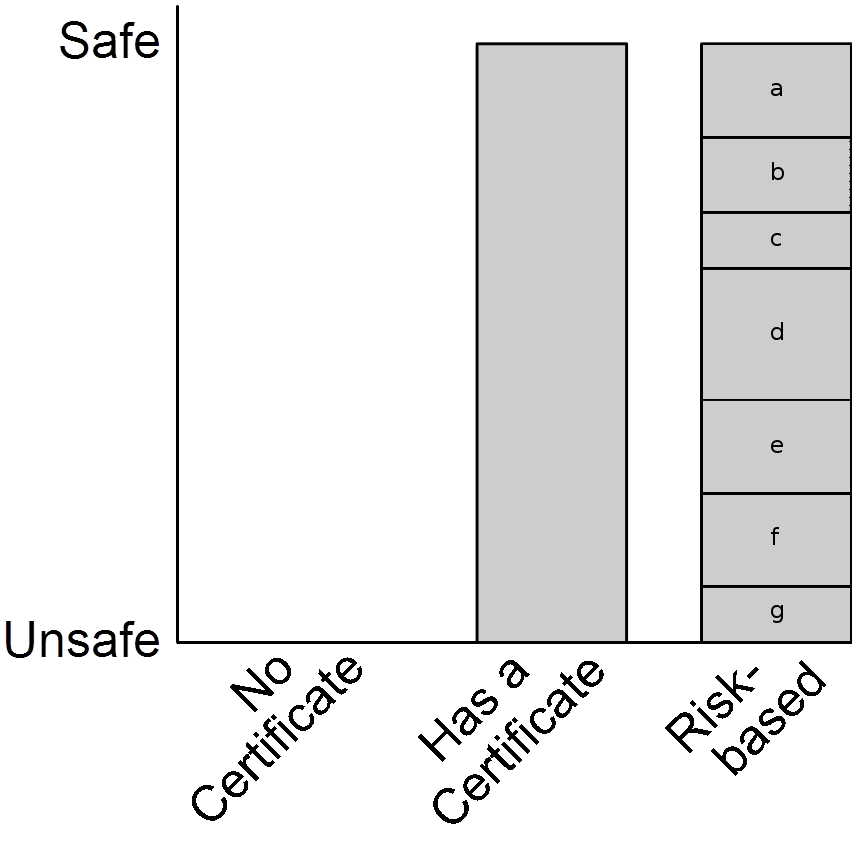
\includegraphics[width=8cm]{Hlebnikov7.png}
  \caption{Пример оценки безопасности Web-сайта при использовании управления рисками}
  \label{Hlebnikov7}
\end{figure}
\end{center}

\end{document}
